
%(BEGIN_QUESTION)
% Copyright 2010, Tony R. Kuphaldt, released under the Creative Commons Attribution License (v 1.0)
% This means you may do almost anything with this work of mine, so long as you give me proper credit

\noindent
{\bf Programming Challenge -- Traffic light controller} 

\vskip 10pt

Write your own PLC program to sequence a single traffic light (green, yellow, and red lights).  The green light should remain on for 15 seconds, the yellow light for 3 seconds, and the red light for 20 seconds.

\vskip 20pt \vbox{\hrule \hbox{\strut \vrule{} {\bf Suggestions for Socratic discussion} \vrule} \hrule}

\begin{itemize}
\item{} Although a sequencing instruction is perhaps the most obvious way to perform this function, is there a way to sequence the traffic light {\it without} using a sequencing instruction?
\end{itemize}

\vfil

\noindent
PLC comparison:

\begin{itemize}
\item{} \underbar{Allen-Bradley Logix 5000}: relevant ladder-logic commands include {\tt SQI}, {\tt SQO}, and {\tt SQL}.
\vskip 5pt
\item{} \underbar{Allen-Bradley SLC 500}: relevant ladder-logic commands include {\tt SQI}, {\tt SQO}, {\tt SQC}, and {\tt SQL}. 
\vskip 5pt
\item{} \underbar{Siemens S7-200}: relevant ladder-logic commands include {\tt SCR}, {\tt SCRE}, and {\tt SCRT}.
\vskip 5pt
\item{} \underbar{Koyo (Automation Direct) DirectLogic}: relevant ladder-logic commands include {\tt DRUM} and {\tt EDRUM}.
\end{itemize}

\underbar{file i02388}
\eject
%(END_QUESTION)





%(BEGIN_ANSWER)


%(END_ANSWER)





%(BEGIN_NOTES)

$$\includegraphics[width=15.5cm]{i02388x01.eps}$$

% No blank lines allowed between lines of an \halign structure!
% I use comments (%) instead, so that TeX doesn't choke.

$$\vbox{\offinterlineskip
\halign{\strut
\vrule \quad\hfil # \ \hfil & 
\vrule \quad\hfil # \ \hfil \vrule \cr
\noalign{\hrule}
%
% First row
Register & Contents \cr
%
\noalign{\hrule}
%
% Another row
{\tt B3:1} & 0000000000000001 \cr
%
\noalign{\hrule}
%
% Another row
{\tt B3:2} & 0000000000000010 \cr
%
\noalign{\hrule}
%
% Another row
{\tt B3:3} & 0000000000000100 \cr
%
\noalign{\hrule}
%
% Another row
{\tt N7:1} & 15 \cr
%
\noalign{\hrule}
%
% Another row
{\tt N7:2} & 3 \cr
%
\noalign{\hrule}
%
% Another row
{\tt N7:3} & 20 \cr
%
\noalign{\hrule}
} % End of \halign 
}$$ % End of \vbox



I strongly recommend students save all their PLC programs for future reference, commenting them liberally and saving them with special filenames for easy searching at a later date!

\vskip 10pt

I also recommend presenting these programs as problems for students to work on in class for a short time period, then soliciting screenshot submissions from students (on flash drive, email, or some other electronic file transfer method) when that short time is up.  The purpose of this is to get students involved in PLC programming, and also to have them see other students' solutions to the same problem.  These screenshots may be emailed back to students at the conclusion of the day so they have other students' efforts to reference for further study.


%INDEX% PLC, programming challenge: traffic light controller (simple)

%(END_NOTES)


